\documentclass[11pt]{article}
\usepackage{indentfirst}
\setlength{\parindent}{2em}

% Language setting
\usepackage[english]{babel}
\usepackage{longtable}
\usepackage{booktabs}
\usepackage{amsmath}
\usepackage{amssymb}
\usepackage[numbers,sort&compress]{natbib}

\allowdisplaybreaks

% Page size and margins
\usepackage[letterpaper,top=2cm,bottom=2cm,left=3cm,right=3cm,marginparwidth=1.75cm]{geometry}

\usepackage{graphicx}
\usepackage[colorlinks=true, allcolors=blue]{hyperref}

\date{}
\title{Project: Static Multi-Trip Routing and Inter-Trip Charging \\
       with Nonlinear Charging and Multi-Station Choice}
\author{Yang Li, Xiao Li}

\begin{document}
\maketitle

\begin{abstract}
\noindent
Electrified-Autonomous Flexible Transit (E-AFT) couples passenger routing with battery management, and most existing formulations either assume constant-rate charging or restrict charging to a single depot. This project formulates a static multi-trip routing and inter-trip charging problem for an E-AFT fleet with multi-station choice, implements it as a single mixed-integer program, and compares a linear charging assumption against a nonlinear tapering charging approximation. Because the bilinear form \(E_{ksr}=p_{ksr}\theta_{ksr}\) in the original formulation is not directly tractable inside the integrated MIP, we replace it with a station-specific piecewise-linear mapping from charging time to charged energy, guarded by indicator constraints. The implementation also uses per-constraint tightened big-\(M\) coefficients, a hierarchical multi-objective (profit primary, completion time secondary), lex-order symmetry breaking across identical buses, and treats the initial dispatch station as a decision variable. Computational experiments on synthetic instances show that in loose cases the two charging assumptions agree on revenue but the nonlinear curve completes the same recharge in roughly a third less charging time, in the partial-recharge scenario the nonlinear model serves one extra request and yields a \(+76.99\) gap in operating profit over the linear plan, and in the deep-recharge scenario both models converge once the instance size available under the size-limited Gurobi license no longer admits a sixth request. The qualitative conclusion is that charging realism changes \emph{which requests are served}, not merely the amount of charging time, and its effect on the operating plan is state-dependent rather than monotone.
\end{abstract}

\section{Problem Description}

Electrified-Autonomous Flexible Transit (E-AFT) is an emerging and promising transportation mode for passenger travel. It allows passengers to submit travel requests online before traveling. They can detail their travel origins, destinations, and acceptable pickup time. Based on passenger requests, E-AFT routes are generated by selecting the appropriate stops to pick up and drop off passengers. Compared to traditional electric buses, E-AFT has a limited battery capacity that constrains traveling range. The smaller battery capacities make them more sensitive to routing planning to serve passenger requests, which requires further research on the optimization of transportation routing planning. In addition, the majority of current research assumes charging only happens at fixed depots \cite{gao2025integrated}. Based on these research gaps, Jiang et al. (2026) \cite{jiang2026two} developed a two-stage optimization approach for dynamic routing and charging scheduling. They assume that charging is restricted to happen between trips where no passengers are on board. They also assume a linear charging speed for vehicle charging. However, the charging speed can be nonlinear in reality \cite{yi2025charging, montoya2017electric}. Building on \cite{jiang2026two}, this project explores a static version of the trip routing and charging scheduling problem with a nonlinear charging profile and an explicit choice among multiple charging stations. The setting is illustrated in Figure~\ref{fig:concept}. Each bus moves from one stop to another to pick up and drop off passengers, which forms a trip. After all passengers drop off, the bus moves to a charging station to recharge. It then moves to the first bus stop of the next trip. The objective is to decide which passenger requests will be served by each bus, along with the route each bus follows within energy-consumption constraints. The nonlinear aspect of the project arises from the charging process, where the charging rate varies with the battery state instead of remaining constant. As a result, routing, timing, and charging decisions are tightly coupled.

\begin{figure}[ht]
    \centering
    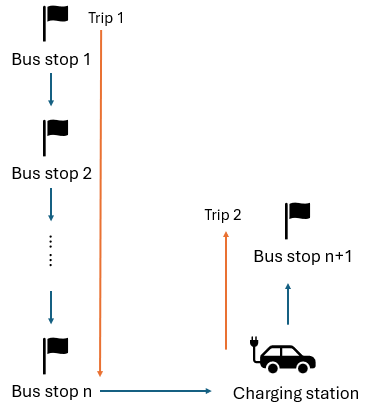
\includegraphics[width=0.55\linewidth]{figures/Figure1.png}
    \caption{Trip routing and inter-trip charging process.}
    \label{fig:concept}
\end{figure}

\section{Mathematical Formulation}

Mathematical notation is summarized in Table~\ref{tab:notation}. Compared with the current study \cite{jiang2026two}, this project focuses on a static version in which routing and charging decisions are optimized once for the entire planning horizon. Instead of solving the problem in two heuristic stages, we formulate it in one optimization problem. In addition, this project examines the situation where the charging speed is nonlinear. For simplicity, several components of the original setting are omitted.

The objective function is the operational profit. It includes the revenue from served passenger requests, the fixed vehicle deployment cost, the penalty cost for unserved requests, the routing cost, and the charging cost.

Constraints (2) and (3) describe whether each request is served by a vehicle or not served. Constraints (4) and (5) ensure that the trip is formed, as at least one request is served during the trip. A subsequent trip can only be formed after the current trip is formed. Constraints (6)--(9) ensure that the pick-up and drop-off nodes are visited exactly once if the request is assigned to the trip. Constraint (10) ensures the flow conservation inside each trip. Constraints (11)--(14) define the first and the last node visited in trips by node connections. When there is no incoming arc for a node that is in the trip, it is the first node visited in the trip. If there is no outgoing arc for a node that is in the trip, it is the last node visited in the trip. Constraints (15)--(18) describe time constraints. Constraints (15) and (16) ensure that the arrival time at the pick-up node is within the acceptable time range. Constraint (17) ensures the drop-off time is later than the pick-up time. Constraint (18) describes within-trip time propagation. Constraints (19)--(21) represent the passenger-load changes as the bus picks up and drops off passengers along the way. Constraints (22)--(25) enforce the trip start and end time to equal the arrival time of the first and the last node of the trip. Constraint (26) ensures the arrival time of the starting node of the next trip is later than the arrival time of the last node of the current trip, plus the time traveling between nodes and a charging station, and the charging duration. Constraints (27) and (28) represent the change in battery level. Constraints (29)--(33) represent trip-level battery boundary constraints. Constraint (34) ensures that charging happens only between trips. Constraint (35) presents the relationship between charging power and charging time. Constraints (36) and (37) define the battery-level transitions between trips. Constraints (38)--(40) apply battery boundaries to the battery level along the trip. Constraints (41)--(51) pertain to the binary or non-negative variables. Among these constraints, (35) is a bilinear form that is naturally nonlinear, and the charging power \(p_{ksr}\) can itself be nonlinear.

\renewcommand{\arraystretch}{1.2}

\begin{longtable}{ll}
\caption{Summary of Notations}
\label{tab:notation} \\
\toprule
\textbf{Symbol} & \textbf{Description} \\
\midrule
\endhead

\multicolumn{2}{l}{\textit{\textbf{Sets and indices}}} \\

$K$ & Set of buses, index $k$ \\
$Q$ & Set of requests, index $q$ \\
$R$ & Set of trip slots for each bus, index $r$ \\
$N^o$ & Set of pickup nodes $\{q^o:q\in Q\}$ \\
$N^d$ & Set of drop-off nodes $\{q^d:q\in Q\}$ \\
$N$ & Set of service nodes $N^o \cup N^d$, index $i,j$ \\
$S$ & Set of charging stations, index $s$ \\

\multicolumn{2}{l}{\textit{\textbf{Parameters}}} \\

$C_m$ & Revenue per served request, \$ \\
$C_v$ & Fixed deployment cost per bus, \$ \\
$C_d$ & Travel cost per unit time, \$/min \\
$C_z$ & Penalty cost per unserved request, \$ \\
$C_e$ & Unit charging cost, \$/min \\
$C_b$ & Bus capacity \\
$\overline{L}$ & Battery capacity, kWh \\
$\underline{L}$ & Minimum battery level, kWh \\
$L_k^0$ & Initial battery level of bus $k$, kWh \\
$t_{1,q}$ & Earliest pickup time of request $q$ \\
$t_{2,q}$ & Latest pickup time of request $q$ \\
$\delta_q$ & Direct in-vehicle service time for request $q$, min \\
$n_q$ & Number of passengers in request $q$ \\
$\tau_{ij}$ & Travel time from node $i$ to node $j$, min \\
$e_{ij}$ & Energy consumption from node $i$ to node $j$, kWh \\
$\tau^0_{ki}$ & Travel time from bus $k$ initial location to node $i$, min \\
$e^0_{ki}$ & Energy consumption from bus $k$ initial location to node $i$, kWh \\
$\tau^{\text{end}}_{is}$ & Travel time from service node $i$ to charging station $s$, min \\
$e^{\text{end}}_{is}$ & Energy consumption from service node $i$ to charging station $s$, kWh \\
$\tau^{\text{start}}_{si}$ & Travel time from charging station $s$ to service node $i$, min \\
$e^{\text{start}}_{si}$ & Energy consumption from charging station $s$ to service node $i$, kWh \\
$M$ & Sufficiently large positive number \\

\multicolumn{2}{l}{\textit{\textbf{Variables}}} \\

$l^{\text{first}}_{kir} \in \{0,1\}$ & Equals 1 if node $i$ is the first visited service node of bus $k$ in trip $r$ \\
$l^{\text{last}}_{kir} \in \{0,1\}$ & Equals 1 if node $i$ is the last visited service node of bus $k$ in trip $r$ \\
$y_{kqr} \in \{0,1\}$ & Equals 1 if bus \(k\) serves request \(q\) in trip \(r\) \\
$x_{kijr} \in \{0,1\}$ & Equals 1 if bus \(k\) traverses from \(i\) to \(j\) during trip \(r\) \\
$u_{kr} \in \{0,1\}$ & Equals 1 if bus \(k\) operates trip \(r\) \\
$y_q \in \{0,1\}$ & Equals 1 if request \(q\) is served \\
$v_{kir} \in \{0,1\}$ & Equals 1 if node \(i\) is visited by bus \(k\) in trip \(r\) \\
$a_{kir} \ge 0$ & Arrival time of bus \(k\) at node \(i\) in trip \(r\) \\
$w_{kir} \ge 0$ & Onboard passenger load of bus \(k\) after node \(i\) in trip \(r\) \\
$T^{\mathrm{start}}_{kr} \ge 0$ & Start time of trip \(r\) of bus \(k\) \\
$T^{\mathrm{end}}_{kr} \ge 0$ & End time of trip \(r\) of bus \(k\) \\
$L^{\mathrm{start}}_{kr} \ge 0$ & Battery level of bus \(k\) at start of trip \(r\), kWh \\
$L^{\mathrm{end}}_{kr} \ge 0$ & Battery level of bus \(k\) at end of trip \(r\), kWh \\
$L_{kir} \ge 0$ & Battery level of bus \(k\) after visiting node \(i\) in trip \(r\), kWh \\
$z_{ksr} \in \{0,1\}$ & Equals 1 if bus \(k\) charges at station \(s\) between trips \(r\) and \(r+1\) \\
$\theta_{ksr} \ge 0$ & Charging duration of bus \(k\) at station \(s\) between trips \(r\) and \(r+1\) \\
$p_{ksr} \ge 0$ & Charging power at station $s$, kW \\
$E_{ksr} \ge 0$ & Charged energy of bus \(k\) at station \(s\) between trips \(r\) and \(r+1\), kWh \\

\bottomrule
\end{longtable}

\begin{align}
\max Z
=& \sum_{q\in Q} C_m y_q
-\sum_{k\in K}\sum_{r\in R} C_v u_{kr}
-\sum_{q\in Q} C_z(1-y_q) \notag\\
&-\sum_{k\in K}\sum_{r\in R}\sum_{i\in N}\sum_{j\in N} C_d \tau_{ij} x_{kijr}
-\sum_{k\in K}\sum_{r\in R\setminus\{\max R\}}\sum_{s\in S} C_e E_{ksr}
\tag{1}
\end{align}

s.t.
\begin{align}
y_q= \sum_{k\in K}\sum_{r\in R} y_{kqr},
&& \forall q\in Q
\tag{2}\\
y_q\le 1,
&& \forall q\in Q
\tag{3} \\
y_{kqr}\le u_{kr},
&& \forall k\in K,\; q\in Q,\; r\in R
\tag{4}\\
u_{k,r+1}\le u_{kr},
&& \forall k\in K,\; r\in R\setminus\{\max R\}
\tag{5} \\
\sum_{j\in N} x_{k,q^o,j,r}= y_{kqr},
&& \forall k\in K,\; q\in Q,\; r\in R
\tag{6}\\
\sum_{i\in N} x_{k,i,q^o,r}= y_{kqr},
&& \forall k\in K,\; q\in Q,\; r\in R
\tag{7}\\
\sum_{j\in N} x_{k,q^d,j,r}= y_{kqr},
&& \forall k\in K,\; q\in Q,\; r\in R
\tag{8}\\
\sum_{i\in N} x_{k,i,q^d,r}= y_{kqr},
&& \forall k\in K,\; q\in Q,\; r\in R
\tag{9} \\
\sum_{j\in N} x_{kijr}= \sum_{h\in N} x_{khir},
&& \forall k\in K,\; i\in N,\; r\in R
\tag{10} \\
\sum_{h\in N} x_{khir} + l^{\text{first}}_{kir}= v_{kir},
&& \forall k \in K,\; i \in N,\; r \in R
\tag{11} \\
\sum_{j\in N} x_{kijr} + l^{\text{last}}_{kir}= v_{kir},
&& \forall k \in K,\; i \in N,\; r \in R
\tag{12} \\
\sum_{i\in N} l^{\text{first}}_{kir}= u_{kr},
&& \forall k \in K,\; r \in R
\tag{13} \\
\sum_{i\in N} l^{\text{last}}_{kir}= u_{kr},
&& \forall k \in K,\; r \in R
\tag{14} \\
a_{k,q^o,r}\ge t_{1,q} - M(1-y_{kqr}),
&& \forall k\in K,\; q\in Q,\; r\in R
\tag{15} \\
a_{k,q^o,r}\le t_{2,q} + M(1-y_{kqr}),
&& \forall k\in K,\; q\in Q,\; r\in R
\tag{16} \\
a_{k,q^d,r}\ge a_{k,q^o,r} + \delta_q - M(1-y_{kqr}),
&& \forall k\in K,\; q\in Q,\; r\in R
\tag{17} \\
a_{kjr}\ge a_{kir} + \tau_{ij} - M(1-x_{kijr}),
&& \forall k\in K,\; i,j\in N,\; r\in R
\tag{18} \\
\Delta_i=
\begin{cases}
+n_q, & \text{if } i=q^o,\\
-n_q, & \text{if } i=q^d.
\end{cases}
&& \forall i\in N
\tag{19} \\
w_{kjr}\ge w_{kir} + \Delta_j - M(1-x_{kijr}),
&& \forall k\in K,\; i,j\in N,\; r\in R
\tag{20}\\
0\le w_{kir} \le C_b,
&& \forall k\in K,\; i\in N,\; r\in R
\tag{21} \\
T^{\mathrm{start}}_{kr}\le a_{kir} + M\Bigl(1-l^{\text{first}}_{kir}\Bigr),
&& \forall k\in K,\; i\in N,\; r\in R
\tag{22}\\
T^{\mathrm{start}}_{kr}\ge a_{kir} - M\Bigl(1-l^{\text{first}}_{kir}\Bigr),
&& \forall k\in K,\; i\in N,\; r\in R
\tag{23}\\
T^{\mathrm{end}}_{kr}\ge a_{kir} - M\Bigl(1-l^{\text{last}}_{kir}\Bigr),
&& \forall k\in K,\; i\in N,\; r\in R
\tag{24}\\
T^{\mathrm{end}}_{kr}\le a_{kir} + M\Bigl(1-l^{\text{last}}_{kir}\Bigr),
&& \forall k\in K,\; i\in N,\; r\in R
\tag{25}\\
T^{\mathrm{start}}_{k,r+1}\ge T^{\mathrm{end}}_{kr}
+ \tau^{\mathrm{end}}_{i s}
+ \theta_{ksr}
+ \tau^{\mathrm{start}}_{s j}
- M(1-z_{ksr}),
&& \forall k,s,r
\tag{26} \\
L_{kjr}\le L_{kir} - e_{ij} + M(1-x_{kijr}),
&& \forall k\in K,\; i,j\in N,\; r\in R
\tag{27} \\
L_{kjr}\ge L_{kir} - e_{ij} - M(1-x_{kijr}),
&& \forall k\in K,\; i,j\in N,\; r\in R
\tag{28} \\
L^{\mathrm{end}}_{kr}\ge L_{kir} - M\Bigl(1-l^{\text{last}}_{kir}\Bigr),
&& \forall k\in K,\; i\in N,\; r\in R
\tag{29} \\
L^{\mathrm{end}}_{kr}\le L_{kir} + M\Bigl(1-l^{\text{last}}_{kir}\Bigr),
&& \forall k\in K,\; i\in N,\; r\in R
\tag{30} \\
L^{\mathrm{start}}_{k1}= L_k^0,
&& \forall k\in K
\tag{31} \\
L_{kir}\le L^{\mathrm{start}}_{kr},
&& \forall k\in K,\; i\in N,\; r\in R
\tag{32} \\
L^{\mathrm{end}}_{kr}\le L^{\mathrm{start}}_{kr},
&& \forall k\in K,\; r\in R
\tag{33} \\
\theta_{ksr}\le M z_{ksr},
&& \forall k\in K,\; s\in S,\; r\in R\setminus\{\max R\}
\tag{34}\\
E_{ksr}= p_{ksr}\theta_{ksr},
&& \forall k\in K,\; s\in S,\; r\in R\setminus\{\max R\}
\tag{35} \\
L^{\mathrm{start}}_{k,r+1}=
L^{\mathrm{end}}_{kr}
+ \sum_{s\in S} E_{ksr}
- \sum_{s\in S} \Bigl(e^{\mathrm{dead}}_{ksr} z_{ksr}\Bigr),
&& \forall k\in K,\; r\in R\setminus\{\max R\}
\tag{36} \\
e^{\mathrm{dead}}_{ksr}= \sum_{i\in N}\sum_{j\in N} \Bigl(e^{\text{end}}_{is} + e^{\text{start}}_{sj}\Bigr) l^{\text{last}}_{kir} l^{\text{first}}_{k,j,r+1},
&& \forall k\in K,\; r\in R,\; s\in S
\tag{37} \\
\underline{L}\le L_{kir} \le \overline{L},
&& \forall k\in K,\; i\in N,\; r\in R
\tag{38} \\
\underline{L}\le L^{\mathrm{start}}_{kr} \le \overline{L},
&& \forall k\in K,\; r\in R
\tag{39}\\
\underline{L}\le L^{\mathrm{end}}_{kr} \le \overline{L},
&& \forall k\in K,\; r\in R
\tag{40} \\
x_{kijr}\in \{0,1\},
&& \forall k\in K,\; i,j\in N,\; r\in R
\tag{41}\\
y_{kqr}\in \{0,1\},
&& \forall k\in K,\; q\in Q,\; r\in R
\tag{42}\\
y_q\in \{0,1\},
&& \forall q\in Q
\tag{43}\\
u_{kr}\in \{0,1\},
&& \forall k\in K,\; r\in R
\tag{44}\\
z_{ksr}\in \{0,1\},
&& \forall k\in K,\; s\in S,\; r\in R\setminus\{\max R\}
\tag{45} \\
v_{kir}\in \{0,1\},
&& \forall k\in K,\; i\in N,\; r\in R
\tag{46} \\
a_{kir}\ge 0,
&& \forall k\in K,\; i\in N,\; r\in R
\tag{47}\\
w_{kir}\ge 0,
&& \forall k\in K,\; i\in N,\; r\in R
\tag{48}\\
\theta_{ksr}\ge 0,
&& \forall k\in K,\; s\in S,\; r\in R\setminus\{\max R\}
\tag{49}\\
E_{ksr}\ge 0,
&& \forall k\in K,\; s\in S,\; r\in R\setminus\{\max R\}
\tag{50}\\
T^{\mathrm{start}}_{kr},\; T^{\mathrm{end}}_{kr},\; L^{\mathrm{start}}_{kr},\; L^{\mathrm{end}}_{kr},\; L_{kir} \ge 0,
&& \forall k\in K,\; i\in N,\; r\in R
\tag{51}
\end{align}

\section{Implementation and Simplifications}

We implemented the formulation in Python using the Gurobi solver. Constraint (35), \(E_{ksr}=p_{ksr}\theta_{ksr}\), is a bilinear term with two decision variables and is not directly compatible with a standard MILP solve. Rather than invoking Gurobi's quadratic-constraint machinery inside the integrated model, we replace it with a station-specific piecewise-linear map from the charging duration \(\theta_{ksr}\) to the charged energy \(E_{ksr}\), defined by breakpoints \(\bigl(\theta^{(1)}_s,\ldots,\theta^{(P)}_s\bigr)\) and \(\bigl(E^{(1)}_s,\ldots,E^{(P)}_s\bigr)\). Linear charging corresponds to evenly spaced breakpoints with constant slope; nonlinear (tapering) charging corresponds to concave, decreasing-slope breakpoints where the first segment captures the fast early-charging regime and the last segment captures the slow tail. Station differences are modeled by scaling the time axis of the breakpoints by a station-specific factor, so a ``hub'' station can deliver the same energy in less time than a ``depot.'' Figure~\ref{fig:charging-profiles} shows both curves and the three station-specific variants.

\begin{figure}[ht]
    \centering
    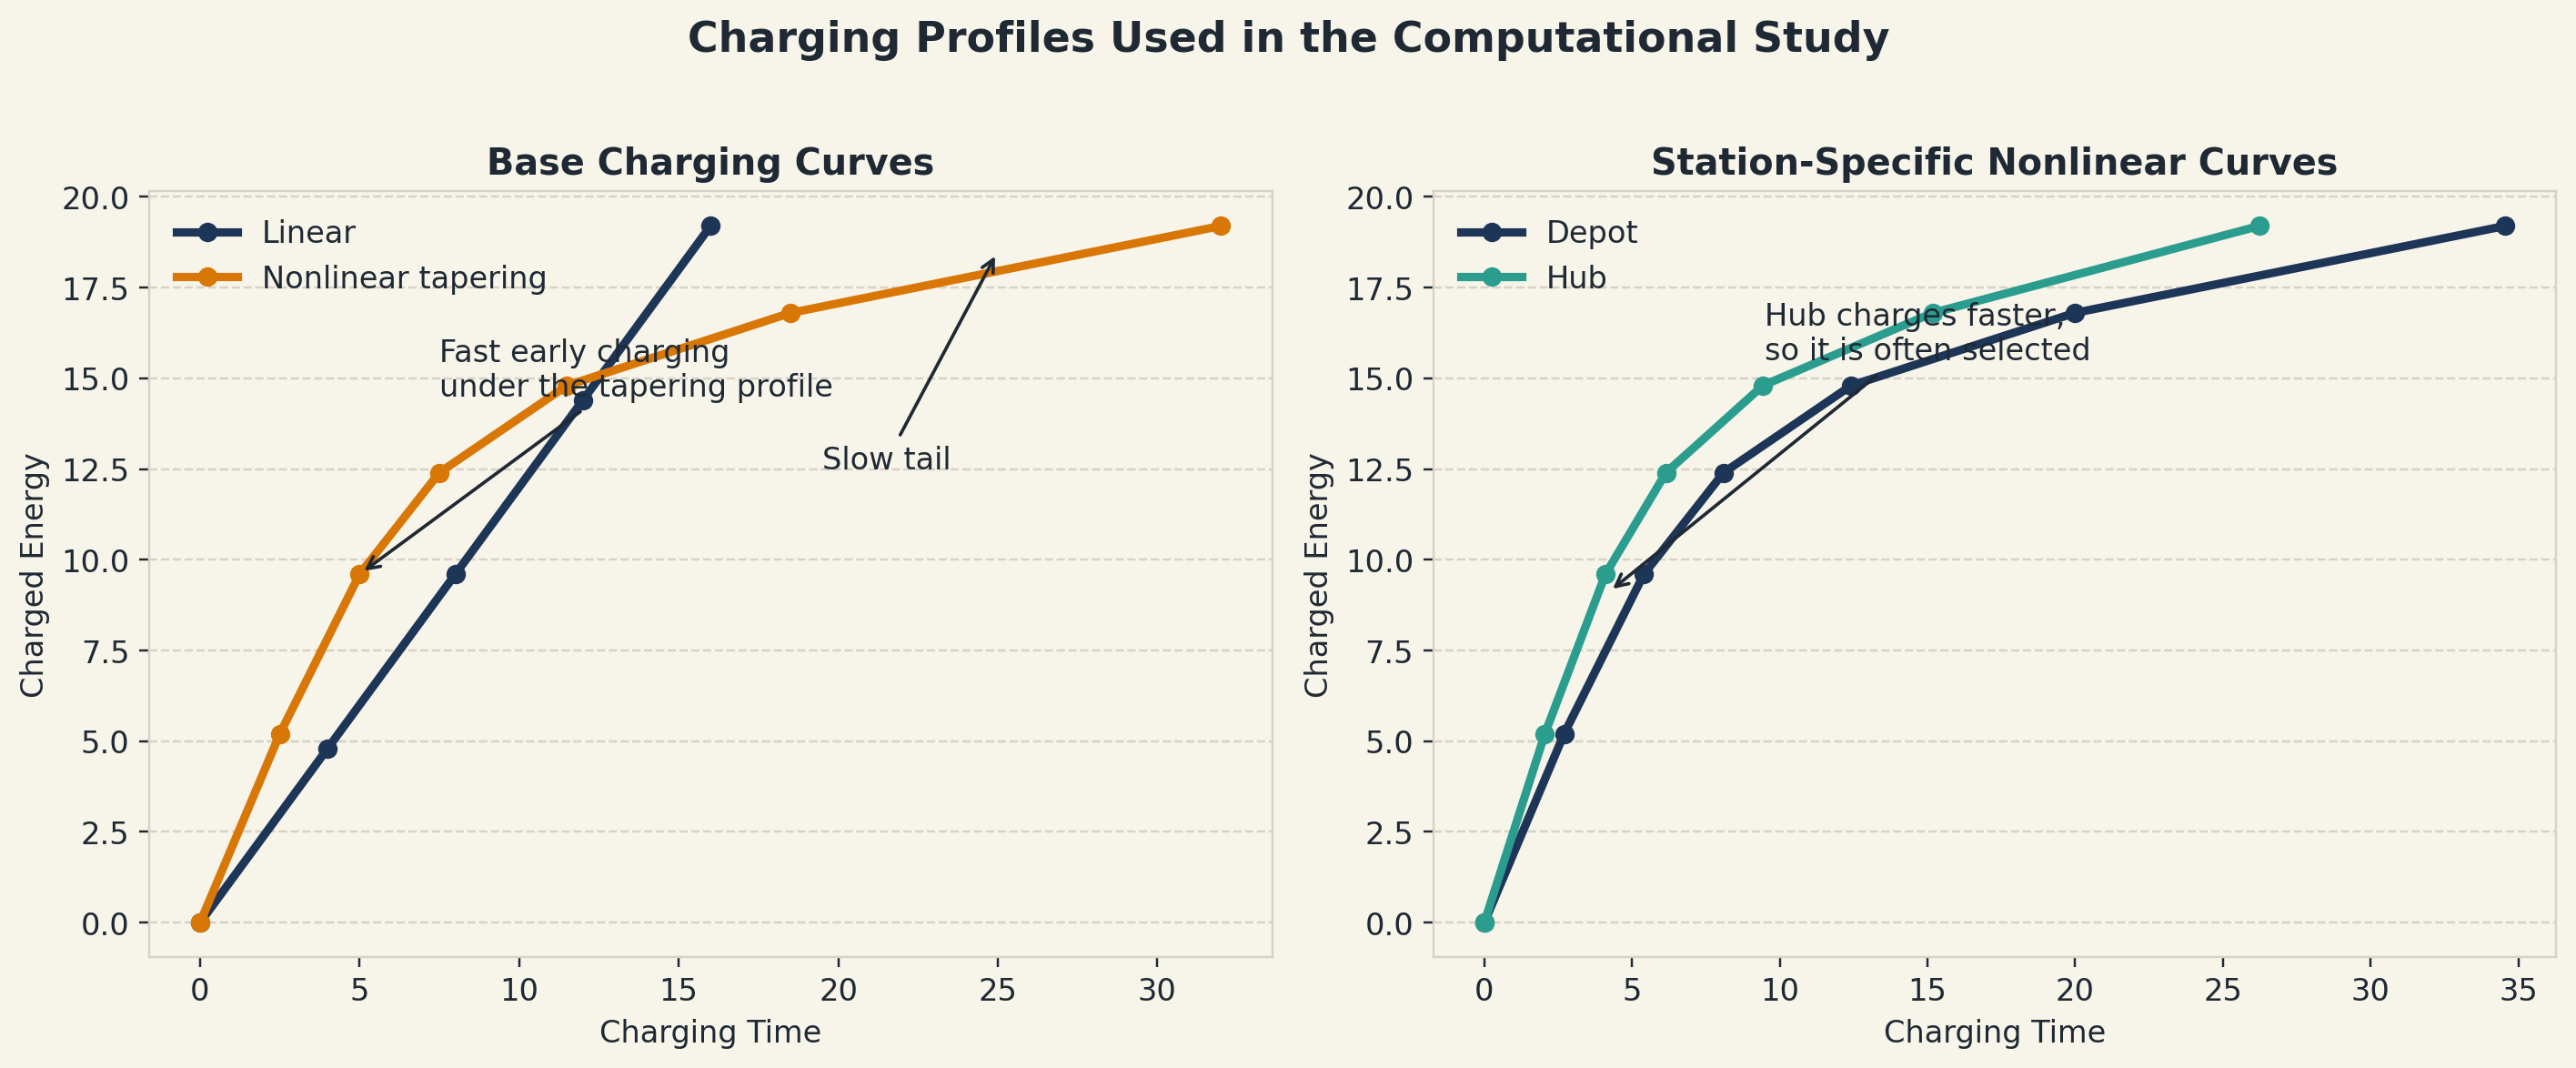
\includegraphics[width=0.95\linewidth]{figures/charging_profiles.png}
    \caption{Charging curves used in the computational study. Left: linear vs.\ nonlinear tapering base curves. Right: station-specific nonlinear curves obtained by scaling the time axis. The hub station charges fastest and is consistently preferred by the solver for the mid-plan recharge.}
    \label{fig:charging-profiles}
\end{figure}

To keep the integrated formulation solvable under a size-limited Gurobi license, the implementation applies several tightening and symmetry reductions. First, the redundant \(v_{kir}\) indicator is eliminated because pickup and drop-off visits are uniquely determined by the assignment variable \(y_{kqr}\). Second, every big-\(M\) coefficient is replaced with the tightest valid bound for that specific constraint family: \(\overline{L}+\max_{ij}e_{ij}\) for battery flow, \(C_b+\max_q n_q\) for load flow, and \(T_{\max}+\theta_{\max}+\tau_{\max}\) for the inter-trip time transition, rather than a single global constant. Third, the piecewise-linear charging relation is wrapped by a Gurobi indicator constraint so that the piecewise map is only active when \(z_{ksr}=1\); when the station is not selected, the charging-time and charging-energy variables are forced to zero and the piecewise model is inert. Fourth, a hierarchical multi-objective is used (profit as primary, total completion time as secondary) so that among profit-equivalent solutions the solver prefers earlier ones, avoiding the numerical fragility of a weighted sum with a tiny tie-break coefficient. Fifth, for instances with more than one bus, the model adds lex-order symmetry-breaking constraints between adjacent buses so that interchangeable permutations of the same solution do not enlarge the branch-and-bound tree. Finally, the initial dispatch station is treated as a decision variable: the first trip of each bus picks its origin station jointly with the rest of the plan, so the solver can co-locate the bus closer to the first pickup cluster when that is optimal.

These changes do not alter the semantics of the formulation; they only change what is tractable to solve. The overall model, including the piecewise charging relation, is still a mixed-integer program with a profit objective, and the experiments in the next section all correspond to instances of this formulation.

\section{Computational Study}

We evaluate the model on synthetic instances sized to fit within the current size-limited Gurobi license (roughly a few hundred variables and constraints). The default configuration uses one bus, two trip slots, two charging stations, and four passenger requests; the deep-recharge scenario uses five requests. Travel times and energy consumption are generated from Euclidean distances on a small synthetic grid.

We evaluate three representative scenarios:
\begin{itemize}
    \item \textbf{Baseline} -- a loose 4-request instance in which both charging models can serve all requests. This is the sanity check.
    \item \textbf{Partial recharge} -- a tighter 4-request instance with shifted time windows, designed so that a \emph{moderate} recharge is sufficient. This scenario is meant to probe whether the tapering curve helps when the bus mainly charges in the fast early portion of the curve.
    \item \textbf{Deep recharge} -- a tighter 5-request instance with further-shifted windows, so that serving an additional trip requires a larger recharge. Originally drafted at 6 requests, this scenario is scaled down here to fit within the size-limited license after the initial-station decision variables were added.
\end{itemize}

\subsection{Direct Comparison of Linear and Nonlinear Charging}

Table~\ref{tab:direct-comparison} summarizes the solver outputs for the three scenarios under both charging assumptions. Figure~\ref{fig:scenario-comparison} plots the same data visually.

\begin{table}[ht]
    \centering
    \small
    \begin{tabular}{lrlrrrrr}
        \toprule
        Scenario & Reqs. & Mode & Objective (\$) & Served & Trips & Charge Time & Charge Energy \\
        \midrule
        Baseline         & 4 & Linear    & 202.98 & 4 & 2 & 6.95 & 10.17 \\
        Baseline         & 4 & Nonlinear & 202.98 & 4 & 2 & 4.52 & 10.17 \\
        Partial recharge & 4 & Linear    & 125.99 & 3 & 2 & 2.29 & 3.35  \\
        Partial recharge & 4 & Nonlinear & 202.98 & 4 & 2 & 4.52 & 10.17 \\
        Deep recharge    & 5 & Linear    & 184.98 & 4 & 2 & 6.95 & 10.17 \\
        Deep recharge    & 5 & Nonlinear & 184.98 & 4 & 2 & 4.52 & 10.17 \\
        \bottomrule
    \end{tabular}
    \caption{Direct comparison of the linear and nonlinear charging assumptions across the three scenarios. Charging time is in time units; charging energy is in kWh.}
    \label{tab:direct-comparison}
\end{table}

\begin{figure}[ht]
    \centering
    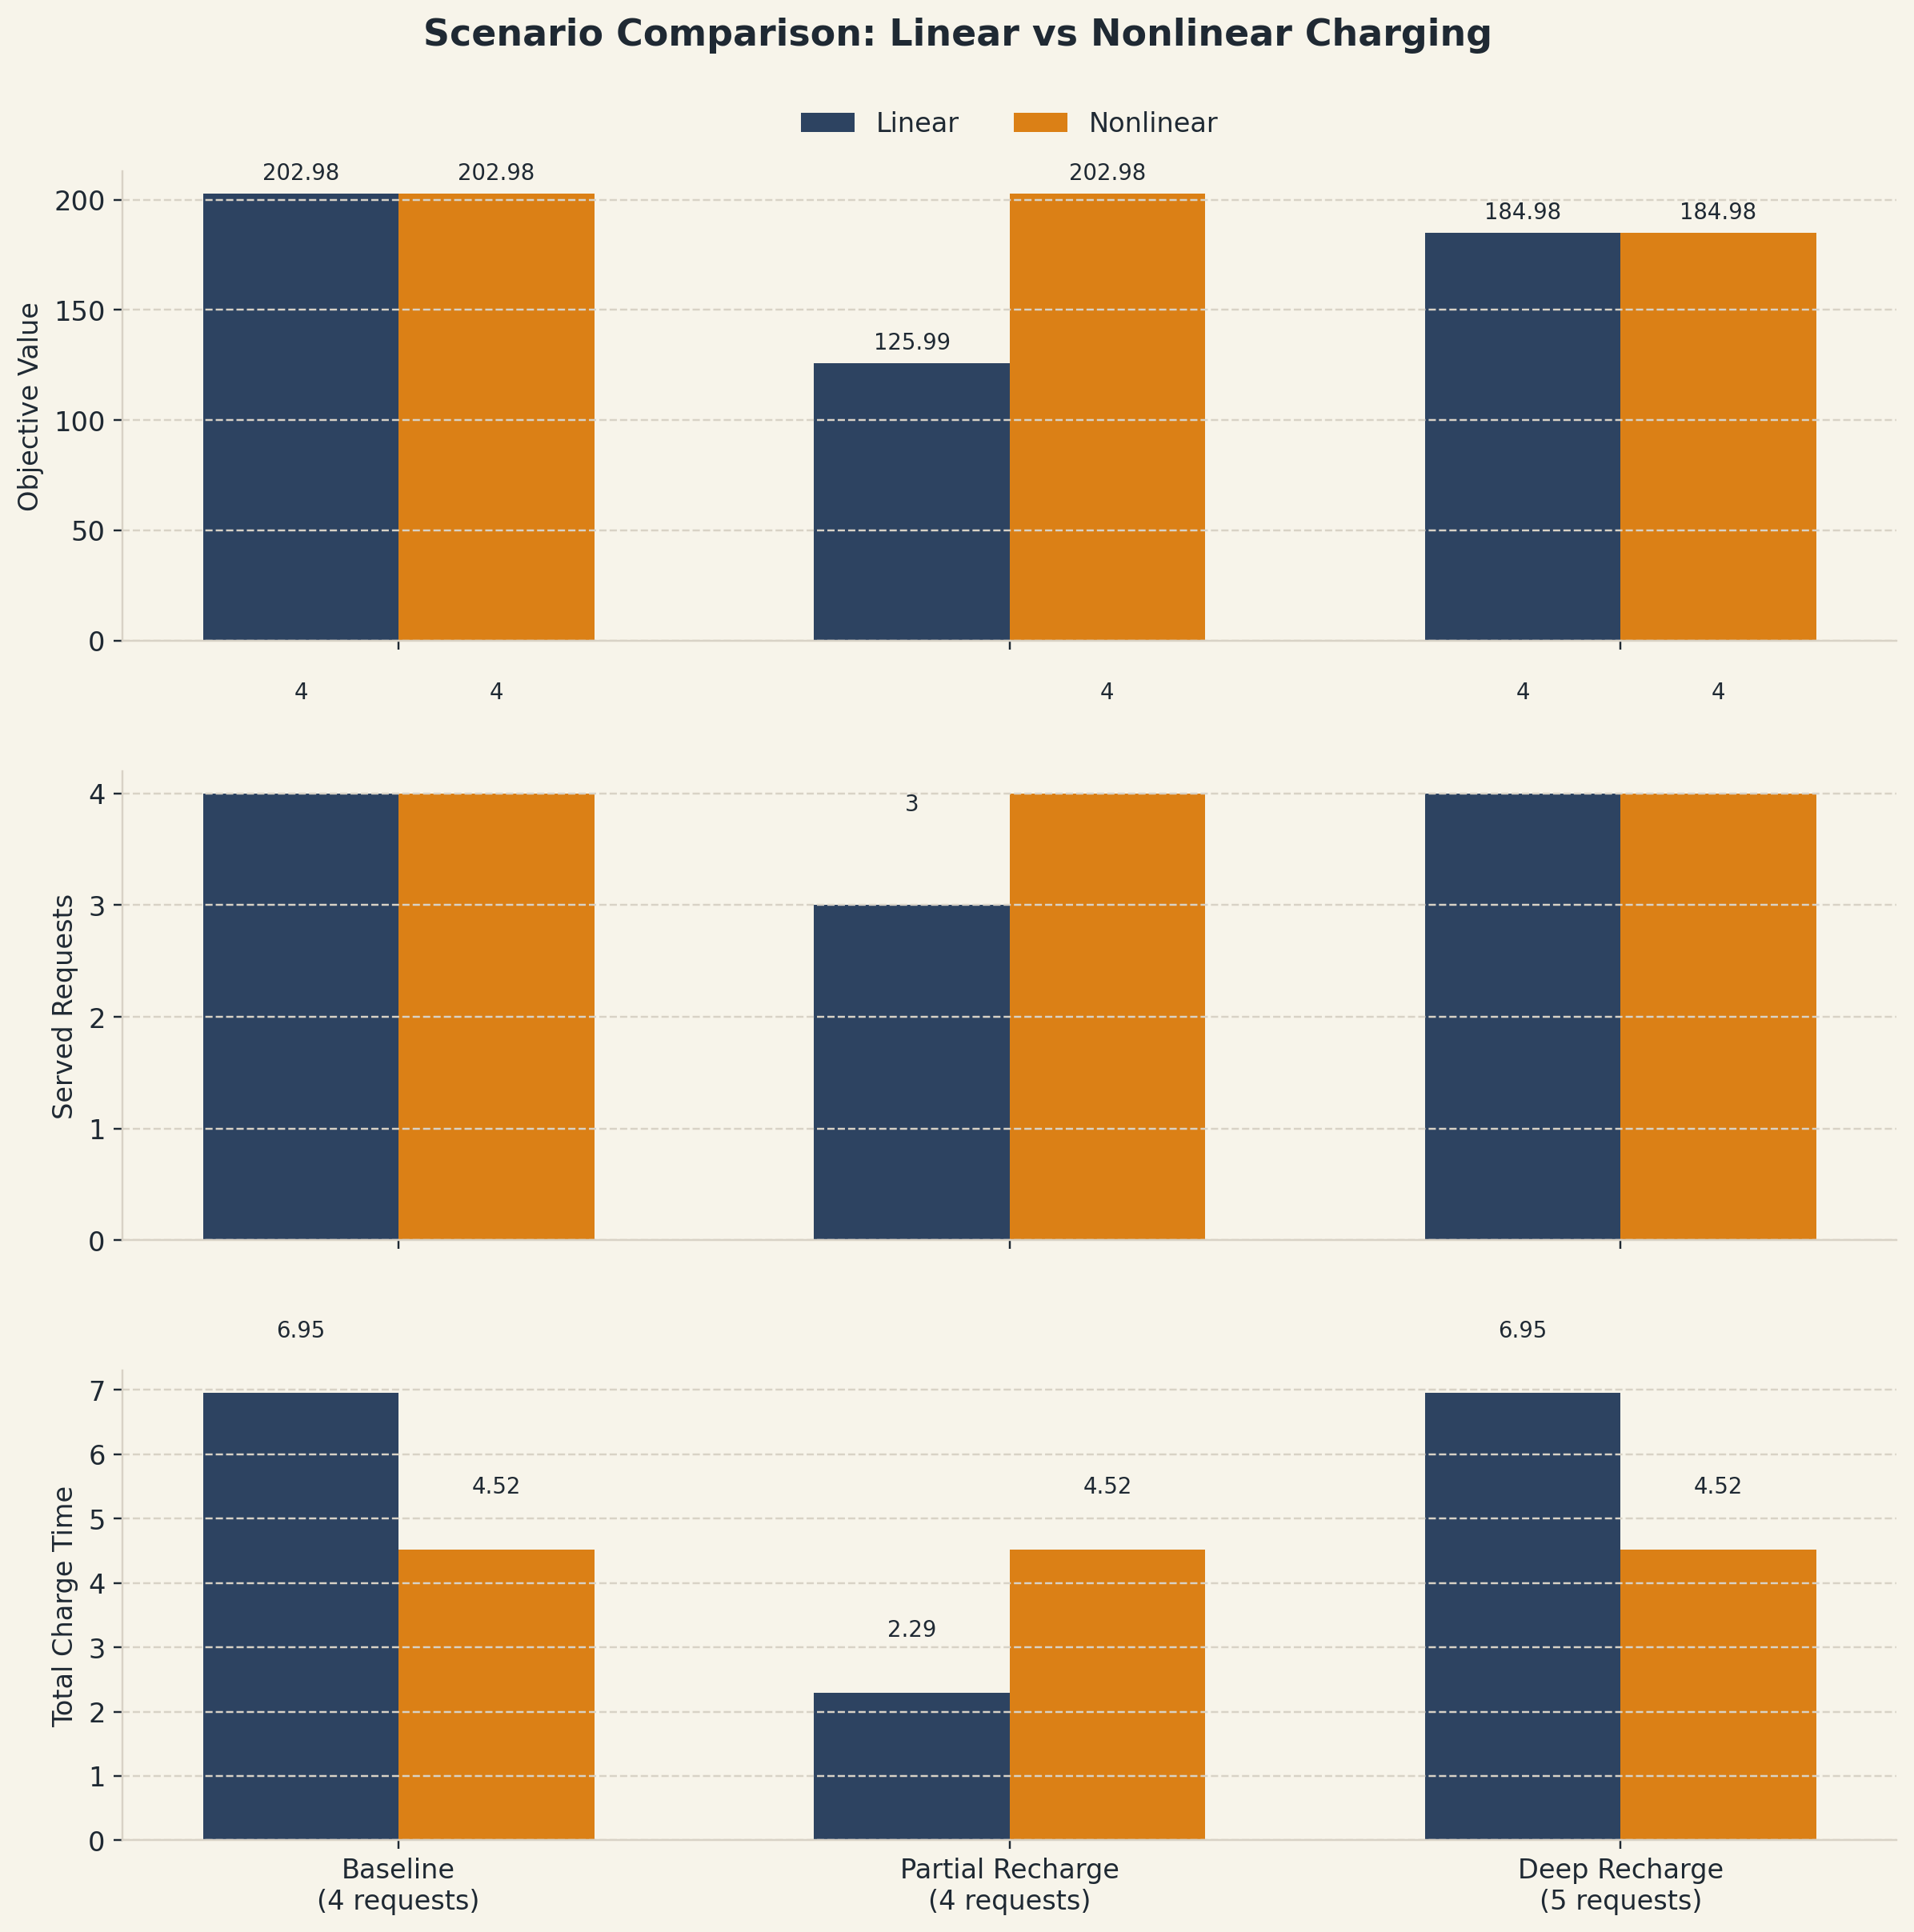
\includegraphics[width=0.9\linewidth]{figures/scenario_comparison.png}
    \caption{Direct comparison of the linear and nonlinear charging models across the main scenarios. The baseline is the same under both assumptions, while the partial-recharge case shows a large gap in objective and in the number of served requests.}
    \label{fig:scenario-comparison}
\end{figure}

Three observations follow. First, in the \textbf{baseline} case, both assumptions serve all four requests and produce the same objective (\(202.98\)). The nonlinear model reaches the plan with noticeably less charging time (\(4.52\) vs.\ \(6.95\)) because it can acquire the same amount of energy faster in the early-charging portion of the taper. This is the expected sanity check: when charging is not the binding constraint, the two models agree on revenue but differ on charging effort.

Second, in the \textbf{partial-recharge} case, the nonlinear assumption outperforms the linear one by \textbf{\(+76.99\)} objective units. Under the linear assumption, the solver believes that the second trip needs a long constant-rate recharge and therefore \emph{drops request \(r_4\)} entirely, serving only three requests. Under the nonlinear assumption, knowing it can top up quickly in the early portion of the curve, the solver repacks the trips and serves all four requests. The charging assumption changes \emph{which requests the operator chooses to serve}, not just how much charging happens.

Third, in the \textbf{deep-recharge} case, both assumptions converge on the same objective (\(184.98\)) and the same served-request set (\(r_1\)--\(r_4\), dropping \(r_5\)). Neither model finds the extra fifth request profitable at this size, so the tapering-vs-constant-rate distinction has no operational effect. A sharper contrast would require returning to the original 6-request instance, which is not solvable under the size-limited license after the model gained the initial-station decision layer. The direction of the linear-vs-nonlinear gap is therefore \emph{state-dependent}: it favors nonlinear when only moderate charging is needed, and is indistinguishable when the deep-recharge regime is not reached.

\subsection{Structural Changes in the Optimal Plans}

The charging assumption changes more than the objective value. It also changes the discrete operational plan.

In the \textbf{partial-recharge} scenario:
\begin{itemize}
    \item the linear model serves \(r_1,r_2\) in Trip 1 and \(r_3\) alone in Trip 2, dropping \(r_4\);
    \item the nonlinear model serves \(r_1,r_2\) in Trip 1 and \(r_3,r_4\) in Trip 2 (all four served).
\end{itemize}

In the \textbf{deep-recharge} scenario, both models converge on the same grouping \(\{r_1,r_2\}\) in Trip 1 and \(\{r_3,r_4\}\) in Trip 2, dropping \(r_5\). When the tapering curve helps, it helps by enabling one additional request rather than by rearranging the trip grouping.

\subsection{Station Selection}

The optimization actively selects a charging station between trips \emph{and} an initial dispatch station for the first trip. Across scenarios the solver dispatches from the \texttt{depot} and recharges at the \texttt{hub}; the hub is preferred because it combines favorable repositioning geometry with the fastest charging time factor. This confirms that both station-choice layers are operationally used by the solver, not just decorative.

\subsection{Cross-Evaluation: Is the Linear-Optimal Plan Still Good Under Nonlinear Charging?}

A central question for this project is whether a plan optimized under the simplified linear charging assumption remains operationally valid once the charging process is modeled more realistically. We answer it with a three-step cross-evaluation:
\begin{enumerate}
    \item optimize the discrete plan (routing, trip assignment, charging-station choice) under \textbf{linear} charging;
    \item hold those discrete choices fixed and re-solve the continuous timing and charging variables under \textbf{nonlinear} charging;
    \item fully re-optimize under \textbf{nonlinear} charging and compare.
\end{enumerate}

Figure~\ref{fig:partial-cross} shows this experiment in the partial-recharge scenario. The linear-optimal plan serves \(r_1,r_2\) in Trip 1, recharges at \texttt{hub} for 2.29 time units (3.35 kWh), and serves only \(r_3\) in Trip 2, at objective \(\mathbf{125.99}\). When the same discrete plan is re-evaluated under the nonlinear curve it remains \emph{feasible} at the same objective \(\mathbf{125.99}\): the same amount of energy is still purchased and under the taper it takes only 1.32 time units instead of 2.29. However, because the inherited plan still ignores \(r_4\), that revenue is left on the table. Fully re-optimizing under the nonlinear curve packs both trips harder -- \(r_1,r_2\) in Trip 1 and \(r_3,r_4\) in Trip 2 with a 4.52-unit recharge at \texttt{hub} -- and reaches objective \(\mathbf{202.98}\), a \(+76.99\) gain. The practical reading is not ``the linear plan is infeasible'' but ``the linear plan is safely executable and quietly drops a profitable request that the nonlinear model is willing to serve.''

\begin{figure}[ht]
    \centering
    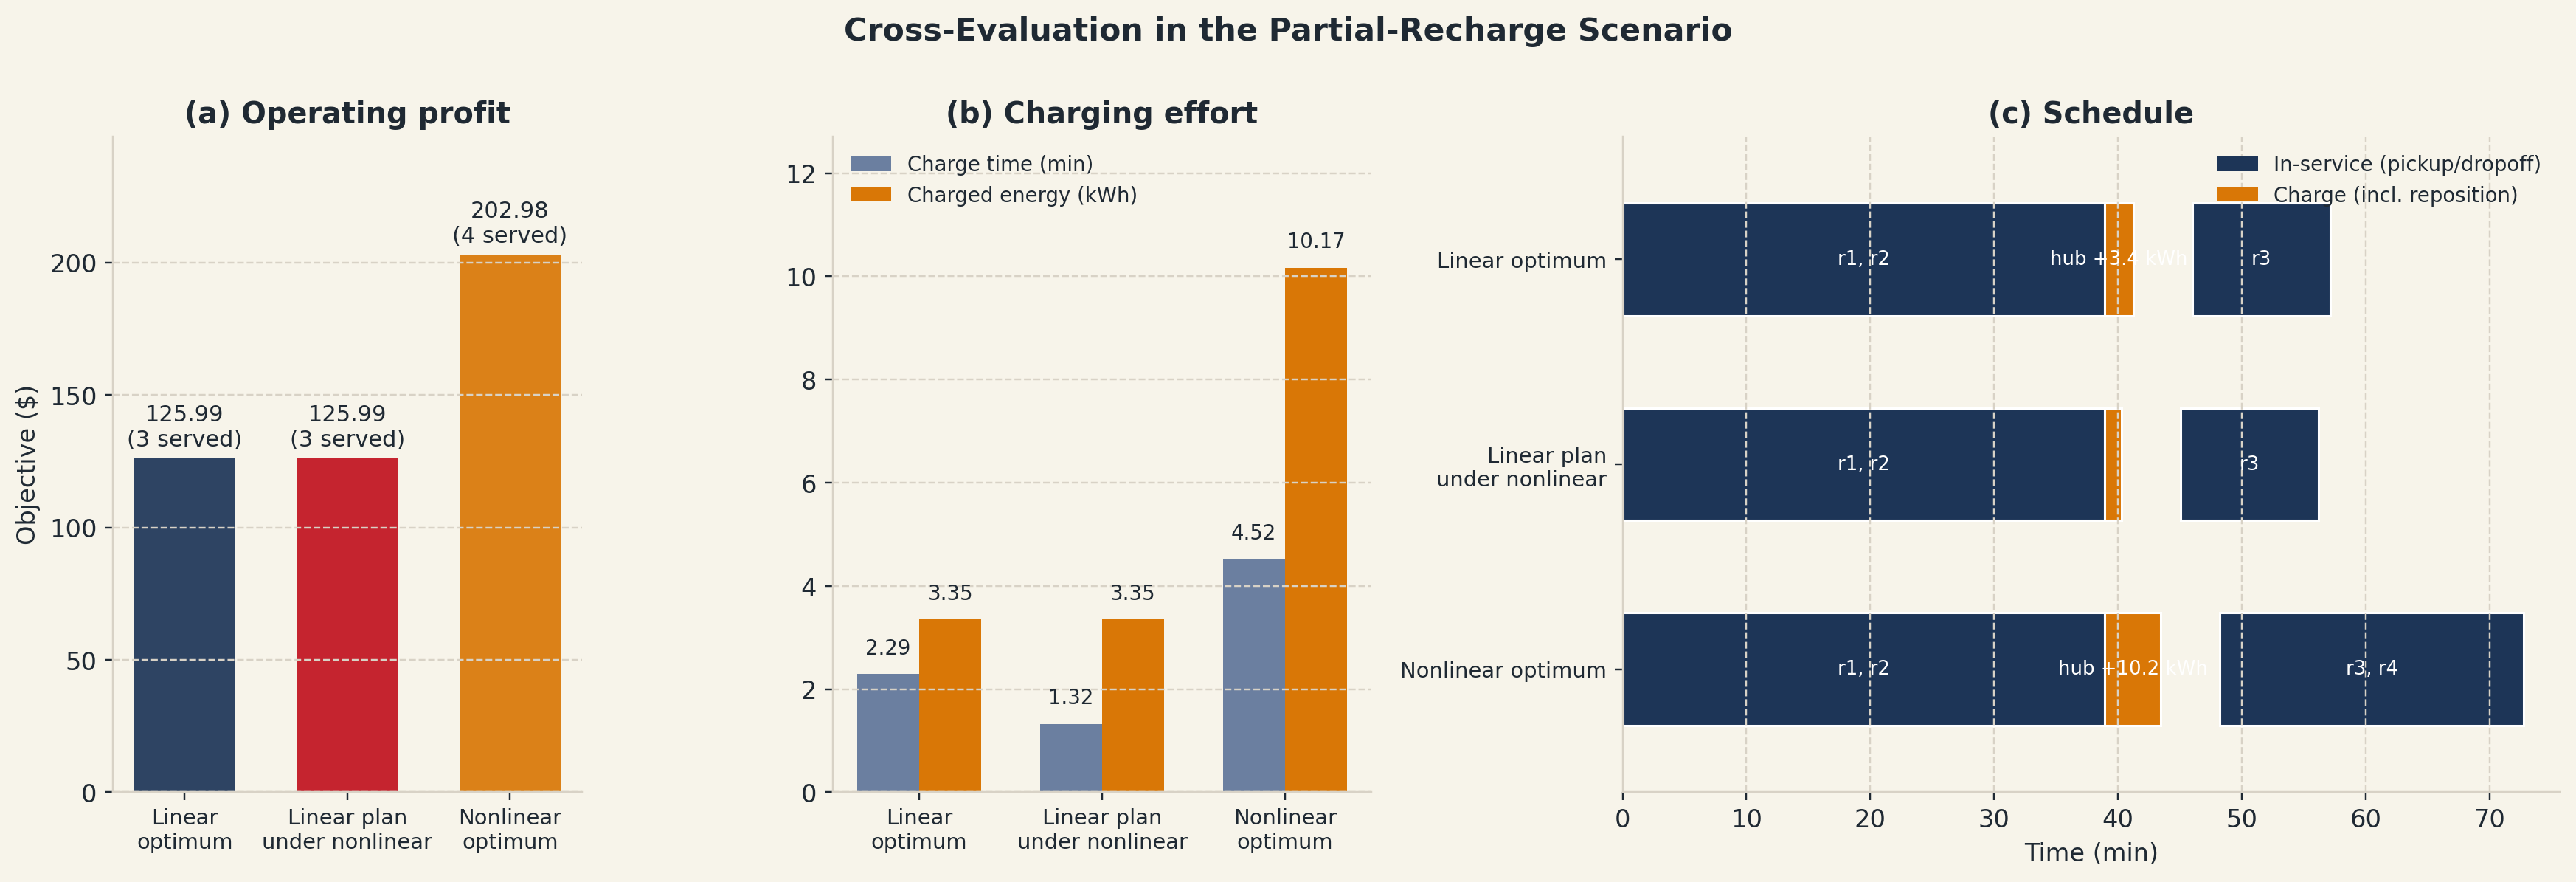
\includegraphics[width=\linewidth]{figures/partial_recharge_cross_evaluation.png}
    \caption{Cross-evaluation in the partial-recharge scenario. The linear-optimal discrete plan remains feasible under the nonlinear charging profile, but leaves \(r_4\) unserved. Re-optimizing under nonlinear charging rebalances the trips and serves all four requests.}
    \label{fig:partial-cross}
\end{figure}

Figure~\ref{fig:deep-cross} shows the corresponding experiment for the deep-recharge scenario at \(R=5\). Here the linear and nonlinear models agree on the discrete plan, and cross-evaluation, as expected, yields the same objective under both charging assumptions. The linear plan is not only feasible under nonlinear charging but also identical in served-request count; the two assumptions differ only in the charging time required to acquire the same energy (4.52 vs.\ 6.95 units). We interpret this as an honest negative result: at this instance size, the cross-evaluation does not exercise the regime in which the linear assumption commits to an unachievable recharge.

\begin{figure}[ht]
    \centering
    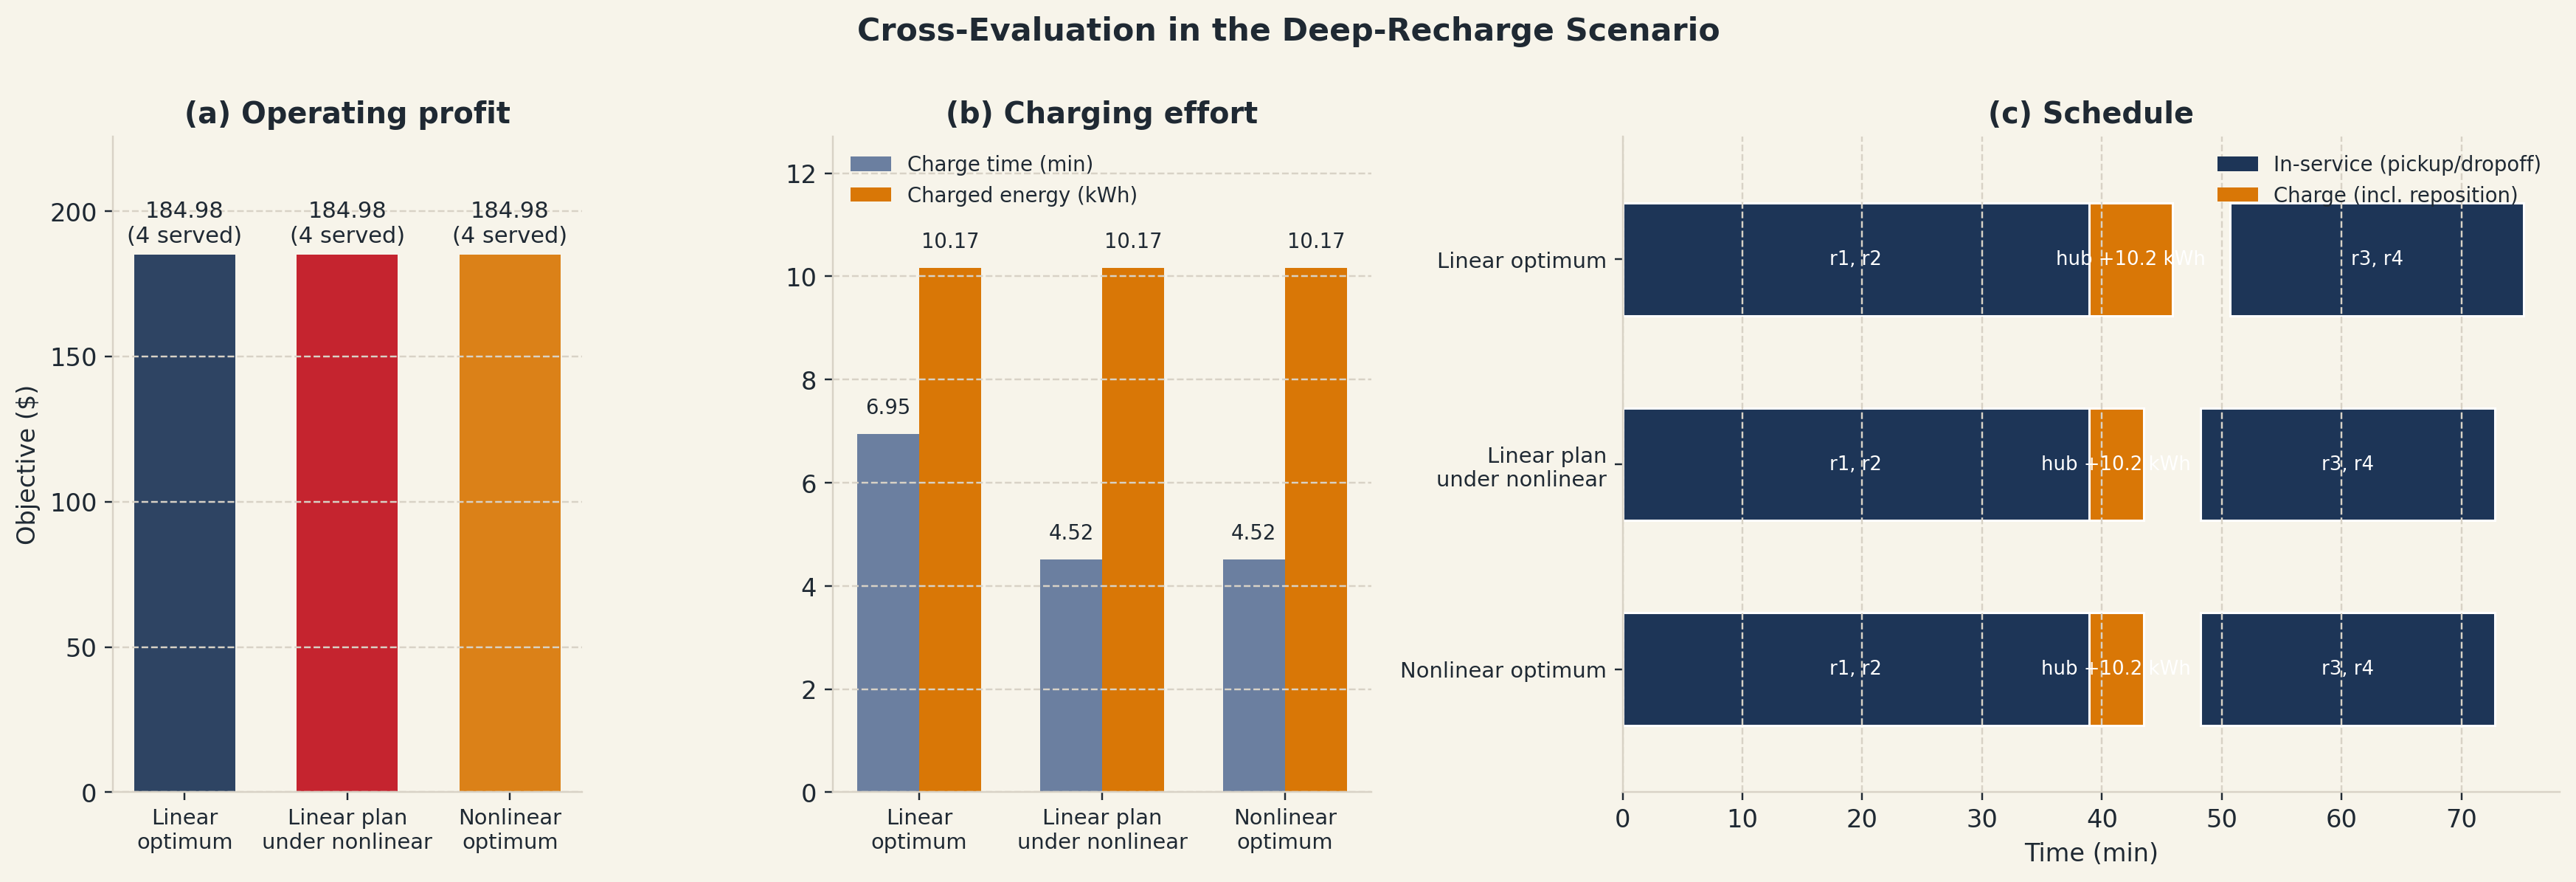
\includegraphics[width=\linewidth]{figures/deep_recharge_cross_evaluation.png}
    \caption{Cross-evaluation in the deep-recharge scenario at \(R=5\). Both charging assumptions reach the same plan and the same objective; only the charging time differs between the two.}
    \label{fig:deep-cross}
\end{figure}

\subsection{Discussion}

Three points summarize what the experiments support. (i) Charging realism is not a cosmetic refinement -- in the partial-recharge regime it changes which requests the operator serves, captures \(+76.99\) in operating profit, and reduces the charging-time footprint by roughly a third for the same amount of energy. (ii) The direction of the effect is state-dependent: if only a moderate recharge is needed, the nonlinear assumption lets the operator be more aggressive; if neither model finds a deeper recharge profitable, the two assumptions are operationally indistinguishable and the linear model is safe to use. (iii) The predicted third regime, in which the linear model is willing to attempt a deeper recharge that the nonlinear model would refuse, is not reached in the instances we can currently solve, because the size-limited Gurobi license no longer admits the originally drafted 6-request deep-recharge case once the richer model (initial-station choice, indicator-guarded PWL, aggregated link variables) is loaded.

\section{Limitations}

The current implementation has several limitations. First, Constraint (35), the bilinear form \(E_{ksr}=p_{ksr}\theta_{ksr}\), is approximated by a piecewise-linear map from charging time to charged energy rather than kept in its original bilinear form; this is what makes the integrated MIP tractable. Second, the test instances are synthetic, generated from a small Euclidean grid, rather than calibrated from real transit operations data. Third, the experiments are intentionally small because of the size-limited Gurobi license; in particular, the deep-recharge story would be sharper at \(R=6\) but that size currently exceeds the license's variable and constraint budget once the initial-station decision layer is included. Fourth, the current model is static: it does not address dynamic arrivals of new requests or stochastic travel times. These are acceptable simplifications for a course project because they allow the project to focus on formulation, implementation, and comparative analysis while keeping the model solvable end-to-end.

\section{Conclusion}

This project develops a tractable mixed-integer optimization model for static multi-trip E-AFT routing with inter-trip charging, explicit multi-station charging choice, and choice of initial dispatch station. The original bilinear charging relation is replaced with a station-specific piecewise-linear charging curve wrapped in an indicator constraint, and the integrated model uses tightened big-\(M\) coefficients, hierarchical multi-objective, and lex-order symmetry breaking.

Across three synthetic scenarios, charging realism is shown to matter in an operationally meaningful way. The two charging assumptions agree on revenue when charging is not binding (baseline), but in the partial-recharge scenario the linear assumption is too conservative -- it drops a profitable request that the nonlinear assumption is willing to serve, opening a \(+76.99\) gap. In the deep-recharge regime at the instance size we can currently solve, both assumptions agree. The effect of charging realism is therefore not monotone: it depends on where the instance sits relative to the threshold at which a deeper recharge becomes marginally profitable. The natural next step, once a larger Gurobi license is available, is to rerun the deep-recharge scenario at \(R=6\) and complete the state-dependent story by observing the third regime, in which the linear model would commit to a recharge that the nonlinear model refuses.

\bibliographystyle{unsrtnat}
\bibliography{sample}

\end{document}
